\documentclass[a4paper, 14pt]{extarticle}

% Поля
%--------------------------------------
\usepackage{geometry}
\geometry{a4paper,tmargin=2cm,bmargin=2cm,lmargin=3cm,rmargin=1cm}
%--------------------------------------

\usepackage{float}
%Russian-specific packages
%--------------------------------------
\usepackage[T2A]{fontenc}
\usepackage[utf8]{inputenc}
\usepackage[english, main=russian]{babel}
%--------------------------------------

\usepackage{textcomp}
\usepackage{xcolor}

% Красная строка
%--------------------------------------
\usepackage{indentfirst}
%--------------------------------------
%Листинги
%--------------------------------------
\usepackage{listings}
\usepackage{listingsutf8}
\lstset{
  basicstyle=\ttfamily\footnotesize,
  breakatwhitespace=false,
  breaklines=true,
  captionpos=t,
  inputencoding=utf8,
  extendedchars=true,
  literate={а}{а}1{б}{б}1{в}{в}1{г}{г}1{д}{д}1{е}{е}1{ё}{ё}1{ж}{ж}1{з}{з}1{и}{и}1{й}{й}1{к}{к}1{л}{л}1{м}{м}1{н}{н}1{о}{о}1{п}{п}1{р}{р}1{с}{с}1{т}{т}1{у}{у}1{ф}{ф}1{х}{х}1{ц}{ц}1{ч}{ч}1{ш}{ш}1{щ}{щ}1{ъ}{ъ}1{ы}{ы}1{ь}{ь}1{э}{э}1{ю}{ю}1{я}{я}1,
  frame=single,
  keepspaces=true,
  keywordstyle=\bf,
  numbers=none,
  xleftmargin=25pt,
  xrightmargin=25pt,
  showspaces=false,
  showstringspaces=false,
  showtabs=false,
  stepnumber=1,
  tabsize=2,
  title=\lstname
}
%--------------------------------------
\usepackage[most]{tcolorbox}
\tcbuselibrary{listings,breakable}
\newtcblisting{breakablelisting}{
  listing only,
  breakable,
  enhanced,
  frame hidden,
  colback=white,
  left=8pt,
  overlay={\draw[line width=0.4pt] (frame.north west) -- (frame.south west);
          \draw[line width=0.4pt] ([xshift=3pt]frame.north west) -- ([xshift=3pt]frame.south west);},
  listing options={
    frame=none,
    numbers=none,
    mathescape=false,
    texcl=false,
    inputencoding=utf8,
    extendedchars=true,
    literate={а}{а}1{б}{б}1{в}{в}1{г}{г}1{д}{д}1{е}{е}1{ё}{ё}1{ж}{ж}1{з}{з}1{и}{и}1{й}{й}1{к}{к}1{л}{л}1{м}{м}1{н}{н}1{о}{о}1{п}{п}1{р}{р}1{с}{с}1{т}{т}1{у}{у}1{ф}{ф}1{х}{х}1{ц}{ц}1{ч}{ч}1{ш}{ш}1{щ}{щ}1{ъ}{ъ}1{ы}{ы}1{ь}{ь}1{э}{э}1{ю}{ю}1{я}{я}1,
    literate={\$}{{\$}}1
  }
}


%Graphics
%--------------------------------------
\usepackage{graphicx}
\usepackage{wrapfig}
%--------------------------------------
\graphicspath{{./lab5/}{./}}
% Полуторный интервал
%--------------------------------------
\linespread{1.3}
%--------------------------------------

%Выравнивание и переносы
%--------------------------------------
% Избавляемся от переполнений
\sloppy
% Запрещаем разрыв страницы после первой строки абзаца
\clubpenalty=10000
% Запрещаем разрыв страницы после последней строки абзаца
\widowpenalty=10000
%--------------------------------------

%Списки
\usepackage{enumitem}

%Подписи
\usepackage{caption}

%Гиперссылки
\usepackage{hyperref}

\hypersetup {
	unicode=true
}

%Рисунки
%--------------------------------------
\DeclareCaptionLabelSeparator*{emdash}{~--- }
\captionsetup[figure]{labelsep=emdash,font=onehalfspacing,position=bottom}
%--------------------------------------

\usepackage{tempora}
\usepackage{tikz}
\usetikzlibrary{arrows.meta,positioning}

%--------------------------------------

%%% Математические пакеты %%%
%--------------------------------------
\usepackage{amsthm,amsfonts,amsmath,amssymb,amscd}  % Математические дополнения от AMS
\usepackage{mathtools}                              % Добавляет окружение multlined
\usepackage[perpage]{footmisc}
%--------------------------------------

%--------------------------------------
%			НАЧАЛО ДОКУМЕНТА
%--------------------------------------

\begin{document}

%--------------------------------------
%			ТИТУЛЬНЫЙ ЛИСТ
%--------------------------------------
\begin{titlepage}
\thispagestyle{empty}
\newpage


%Шапка титульного листа
%--------------------------------------
\vspace*{-60pt}
\hspace{-65pt}
\begin{minipage}{0.3\textwidth}
\hspace*{-20pt}\centering
\includegraphics[width=\textwidth]{emblem}
\end{minipage}
\begin{minipage}{0.67\textwidth}\small \textbf{
\vspace*{-0.7ex}
\hspace*{-6pt}\centerline{Министерство науки и высшего образования Российской Федерации}
\vspace*{-0.7ex}
\centerline{Федеральное государственное автономное образовательное учреждение }
\vspace*{-0.7ex}
\centerline{высшего образования}
\vspace*{-0.7ex}
\centerline{<<Московский государственный технический университет}
\vspace*{-0.7ex}
\centerline{имени Н.Э. Баумана}
\vspace*{-0.7ex}
\centerline{(национальный исследовательский университет)>>}
\vspace*{-0.7ex}
\centerline{(МГТУ им. Н.Э. Баумана)}}
\end{minipage}
%--------------------------------------

%Полосы
%--------------------------------------
\vspace{-25pt}
\hspace{-35pt}\rule{\textwidth}{2.3pt}

\vspace*{-20.3pt}
\hspace{-35pt}\rule{\textwidth}{0.4pt}
%--------------------------------------

\vspace{1.5ex}
\hspace{-35pt} \noindent \small ФАКУЛЬТЕТ\hspace{80pt} <<Информатика и системы управления>>

\vspace*{-16pt}
\hspace{47pt}\rule{0.83\textwidth}{0.4pt}

\vspace{0.5ex}
\hspace{-35pt} \noindent \small КАФЕДРА\hspace{50pt} <<Теоретическая информатика и компьютерные технологии>>

\vspace*{-16pt}
\hspace{30pt}\rule{0.866\textwidth}{0.4pt}

\vspace{11em}

\begin{center}
\Large {\bf Лабораторная работа №2} \\
\large {\bf по курсу <<Моделирование>>} \\
\large <<Оценивание функций связи между ненаблюдаемыми одновременно параметрами>>
\end{center}\normalsize

\vspace{8em}


\begin{flushright}
  {Студент группы ИУ9-82Б Шемякин В.А. \hspace*{15pt}\\
  \vspace{2ex}
  Преподаватель Домрачева А.Б.\hspace*{15pt}}
\end{flushright}

\bigskip

\vfill


\begin{center}
\textsl{Москва 2026}
\end{center}
\end{titlepage}
%--------------------------------------
%		КОНЕЦ ТИТУЛЬНОГО ЛИСТА
%--------------------------------------

\renewcommand{\ttdefault}{pcr}

\setlength{\tabcolsep}{3pt}
\newpage
\setcounter{page}{2}

\section{Постановка задачи}

Цель лабораторной работы заключается в классификации объектов по входным данным из файла \texttt{diabetes.csv} с предварительным выявлением зависимых признаков и последующим сокращением размерности пространства признаков. Тема работы: <<Построение стохастическое модели в заданной предметной области>>.

Для анализа взаимосвязи бинаризованных признаков используются соотношения
\begin{equation}
P(AB)_{\text{завис}} = P(B) \cdot P(A \mid B),
\end{equation}
\begin{equation}
P(AB)_{\text{независ}} = P(A) \cdot P(B).
\end{equation}
Если совместная вероятность ближе к первому выражению, признаки рассматриваются как зависимые; если выполняется второе соотношение, признаки считаются независимыми.

В работе используются столбцы \texttt{Pregnancies}, \texttt{Glucose}, \texttt{BloodPressure}, \texttt{SkinThickness}, \texttt{Insulin}, \texttt{BMI}, \texttt{DiabetesPedigreeFunction}, \texttt{Age} и целевая метка \texttt{Outcome}. Требуется получить компактное представление объектов, снизить размерность задачи, перейти к двум координатам для визуализации и разделить объекты на два класса методом \texttt{k-means}.

Этапы выполнения лабораторной работы следующие:
\begin{enumerate}[label=\arabic*.]
  \item выбор бинаризации показателей;
  \item выбор коэффициента взаимосвязи показателей;
  \item сокращение размерности задачи при наличии зависимых признаков;
  \item кластеризация данных по методу \texttt{k-means};
  \item интерпретация полученных классов по уровням исходных показателей.
\end{enumerate}

\section{Построение модели}

На первом этапе исходные числовые признаки бинаризуются по медианным порогам. Для каждого объекта значение признака заменяется логическим признаком <<выше медианы / не выше медианы>>. В рассматриваемом наборе данных использованы следующие медианы:
\begin{center}
\begin{tabular}{|l|c|l|c|}
\hline
Признак & Медиана & Признак & Медиана \\
\hline
\texttt{Pregnancies} & 3 & \texttt{Insulin} & 30.5 \\
\texttt{Glucose} & 117 & \texttt{BMI} & 32 \\
\texttt{BloodPressure} & 72 & \texttt{DiabetesPedigreeFunction} & 0.3725 \\
\texttt{SkinThickness} & 23 & \texttt{Age} & 29 \\
\hline
\end{tabular}
\end{center}

После бинаризации для каждой пары признаков строятся несколько матриц взаимосвязи. В основном алгоритме используется коэффициент ассоциации, поскольку именно матрица \texttt{association\_matrix.csv} далее загружается в программе и применяется для отбора признаков. Для бинарных показателей такой коэффициент удобен тем, что учитывает согласованность совместных появлений двух высоких или двух низких уровней и принимает значения в диапазоне от $-1$ до $1$.

Сокращение размерности выполняется по следующему правилу. Строится матрица модулей коэффициентов связи, диагональные элементы зануляются, после чего признаки объединяются в компоненты связности при пороге сильной связи $|r| \ge 0.45$. В каждой компоненте в качестве представителя сохраняется признак с максимальной суммарной связью внутри своей группы. По рассчитанной матрице коэффициентов были получены две зависимые группы:
\begin{itemize}
  \item \texttt{Pregnancies}, \texttt{BloodPressure}, \texttt{Age}, из которых сохраняется \texttt{Age};
  \item \texttt{SkinThickness}, \texttt{Insulin}, \texttt{BMI}, из которых сохраняется \texttt{SkinThickness}.
\end{itemize}
Признаки \texttt{Glucose} и \texttt{DiabetesPedigreeFunction} не вошли в группы сильной зависимости и были оставлены без изменений. В результате итоговое пространство признаков для кластеризации имеет четыре координаты: \texttt{Glucose}, \texttt{SkinThickness}, \texttt{DiabetesPedigreeFunction}, \texttt{Age}.

После отбора координат каждый признак стандартизуется, чтобы привести шкалы измерения к сопоставимому виду. Затем на стандартизованных данных выполняется кластеризация методом \texttt{k-means} при $k = 2$. Для графического представления полученного разделения дополнительно применяется проекция главных компонент в двумерное пространство.

Схема построенной модели приведена на рисунке~\ref{fig:model_scheme}.

\begin{figure}[H]
  \centering
  \begin{tikzpicture}[
    node distance=9mm and 7mm,
    block/.style={draw, rounded corners, align=center, minimum width=3.2cm, minimum height=1cm},
    line/.style={-{Latex[length=3mm]}, thick}
  ]
    \node[block] (data) {\texttt{diabetes.csv}};
    \node[block, below=of data] (bin) {Бинаризация\\по медианам};
    \node[block, below=of bin] (assoc) {Матрица коэффициентов\\ассоциации};
    \node[block, below=of assoc] (select) {Отбор независимых\\координат};
    \node[block, below=of select] (std) {Стандартизация};
    \node[block, below=of std] (kmeans) {\texttt{k-means}, $k = 2$};
    \node[block, below left=of kmeans] (pca) {PCA-проекция\\в 2D};
    \node[block, below right=of kmeans] (interpret) {Интерпретация\\классов};

    \draw[line] (data) -- (bin);
    \draw[line] (bin) -- (assoc);
    \draw[line] (assoc) -- (select);
    \draw[line] (select) -- (std);
    \draw[line] (std) -- (kmeans);
    \draw[line] (kmeans) -- (pca);
    \draw[line] (kmeans) -- (interpret);
  \end{tikzpicture}
  \caption{Схема стохастической модели классификации объектов}
  \label{fig:model_scheme}
\end{figure}

\section{Решение вычислительной задачи}

В программе \texttt{main.py} реализован последовательный вычислительный конвейер. Сначала из файла \texttt{diabetes.csv} считываются все числовые признаки, кроме \texttt{Outcome}, и формируется матрица наблюдений. Далее вычисляются медианы и строится бинарное представление признаков. После этого загружается матрица коэффициентов ассоциации \texttt{association\_matrix.csv}, преобразуется в матрицу модулей связей и по порогу $0.45$ выделяются компоненты связности.

Следующий этап состоит в выборе представителей компонент связности. Для каждой группы признаков вычисляется сумма модулей связей внутри группы, после чего сохраняется один представитель. На выбранных четырёх координатах \texttt{Glucose}, \texttt{SkinThickness}, \texttt{DiabetesPedigreeFunction}, \texttt{Age} строится новая матрица признаков, которая затем стандартизуется по среднему значению и среднеквадратическому отклонению.

Кластеризация выполняется методом \texttt{k-means} с параметрами \texttt{k = 2}, \texttt{n\_init = 30}, \texttt{max\_iterations = 300}, \texttt{seed = 42}. Для каждого запуска случайно выбираются начальные центроиды, после чего итерационно пересчитываются принадлежности объектов и центры кластеров. Лучшее разбиение выбирается по минимальному значению внутрикластерной суммы квадратов расстояний. Затем метки кластеров согласуются с \texttt{Outcome} так, чтобы максимизировать долю совпадений. Для визуализации результатов применяется двумерная PCA-проекция стандартизованных точек.

По результатам вычислений были выбраны признаки \texttt{Glucose}, \texttt{SkinThickness}, \texttt{DiabetesPedigreeFunction}, \texttt{Age}. Итоговая точность согласования меток кластеров с \texttt{Outcome} составила $0.7435$. Размеры полученных классов равны: класс~0 содержит 501 объект, класс~1 содержит 267 объектов.

\section{Анализ модели}

Результат кластеризации в двумерной PCA-проекции приведён на рисунке~\ref{fig:clusters}. Изображение отражает не исходное четырёхмерное пространство, а его двумерное представление, используемое только для визуального анализа.

\begin{figure}[H]
  \centering
  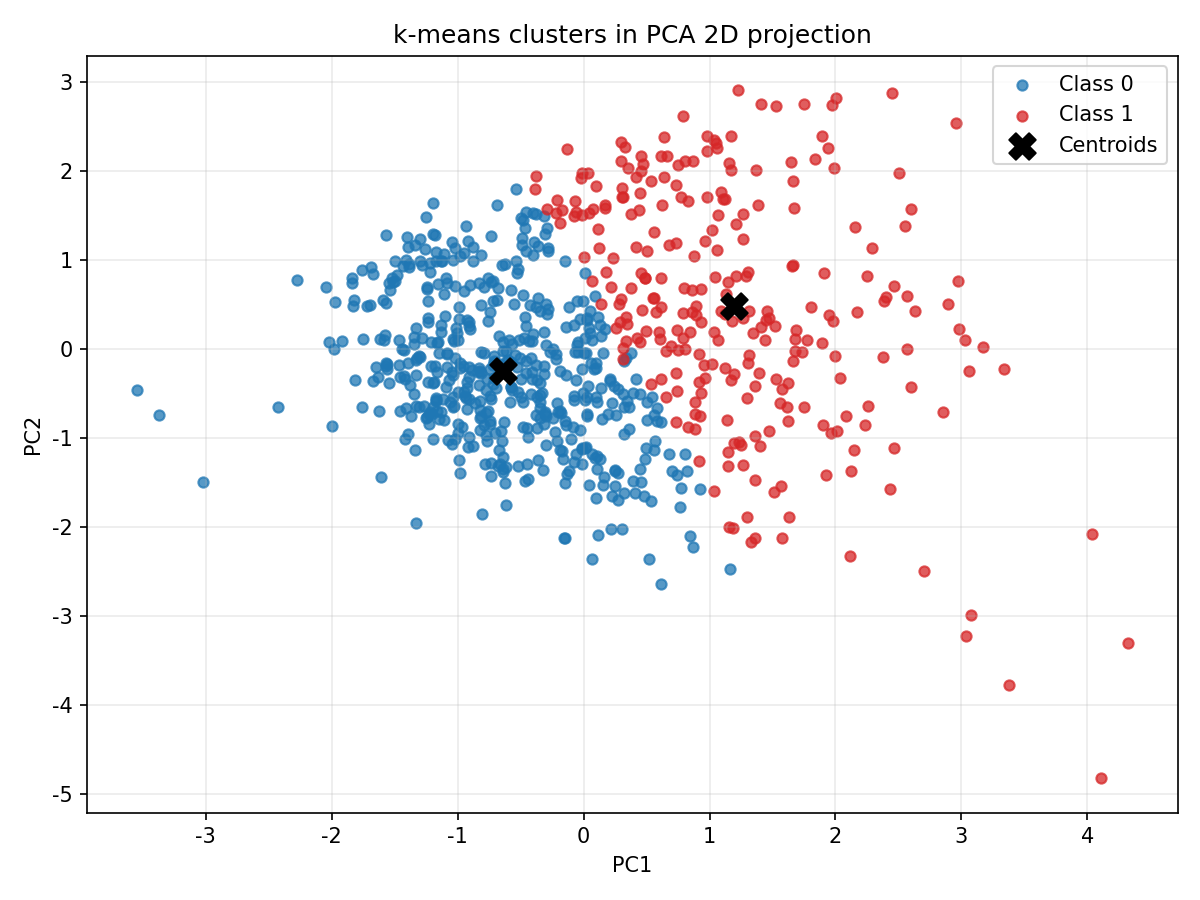
\includegraphics[width=0.8\textwidth]{kmeans_clusters_2d.png}
  \caption{Кластеры объектов в двумерной PCA-проекции}
  \label{fig:clusters}
\end{figure}

Интерпретация классов выполнена по значениям центроидов относительно медиан исходных признаков. Класс~0 включает объекты, для которых \texttt{Glucose} в среднем ниже медианы, \texttt{SkinThickness} ниже медианы, \texttt{DiabetesPedigreeFunction} выше медианы, \texttt{Age} ниже медианы. Класс~1 включает объекты, для которых \texttt{Glucose} выше медианы, \texttt{SkinThickness} ниже медианы, \texttt{DiabetesPedigreeFunction} выше медианы, \texttt{Age} выше медианы.

Сопоставление полученных классов с \texttt{Outcome} показывает, что распределение объектов имеет следующий вид: \texttt{(cluster 0, Outcome 0) = 402}, \texttt{(cluster 0, Outcome 1) = 99}, \texttt{(cluster 1, Outcome 0) = 98}, \texttt{(cluster 1, Outcome 1) = 169}. Следовательно, выбранные признаки и процедура сокращения размерности позволяют получить устойчивое двухклассовое разделение, хотя между классами сохраняется область пересечения.

Содержательно различие классов определяется прежде всего комбинацией уровней \texttt{Glucose} и \texttt{Age}, тогда как \texttt{SkinThickness} в обоих классах остаётся ниже медианного уровня, а \texttt{DiabetesPedigreeFunction} в обоих классах выше медианы. Это означает, что при выбранной модели основной вклад в разделение объектов вносят не все признаки одинаково, а выделенные после сокращения размерности координаты.

\section{Вывод}

В ходе лабораторной работы были выявлены группы зависимых признаков и выполнено сокращение размерности исходного пространства до четырёх координат. На выбранных признаках \texttt{Glucose}, \texttt{SkinThickness}, \texttt{DiabetesPedigreeFunction}, \texttt{Age} метод \texttt{k-means} сформировал два интерпретируемых класса объектов. Согласование кластеров с \texttt{Outcome} дало точность $0.7435$, что показывает пригодность модели для грубой классификации по входным данным. Построенная схема обработки данных позволяет последовательно переходить от анализа связей между признаками к итоговому разбиению объектов на классы.

\section{Практическая реализация}

Листинг~\ref{lst:main_code} содержит исходный код программы, реализующей бинаризацию признаков, отбор зависимых групп, сокращение размерности, кластеризацию и визуализацию результатов.

\lstinputlisting[
  language=Python,
  inputencoding=utf8/latin1,
  caption={Исходный код программы \texttt{main.py}},
  label={lst:main_code}
]{main.py}

\end{document}
